\begin{center}
\textbf{CONVEXIDAD Y OPTIMIZACIÓN}

\textbf{\Large ENTREGA B}

\textbf{ \textbf{Christian Limbert Paredes Aguilera}}
\end{center}
\begin{center}
    Latex Source: \url{https://n9.cl/ua8c3}
\end{center}

\line(1,0){400}

\begin{enumerate}[\bfseries \text{Ejercicio} 1.]

\setcounter{enumi}{2}

\begin{comment}
    % -------------------- Ejercicio 1 -------------------- %
    \item \textbf{\boldmath Se considera el problemas
    $$
    \begin{array}{ll}
	\text{minimiza} & x^2+1\\
	\text{sujeto a} & (x-2)(x-4)\leq 0,
    \end{array}
    $$
    con $x\in \mathbb{R}$.}
    \begin{enumerate}[\bfseries (a)]

	% ---------- (a)
	\item \textbf{\boldmath Describe el conjunto accesible, el valor óptimo y las solución optima.}\\
	

	    \textbf{solución:} El conjunto accesible, esta formado por todos los valores de $x$ que satisfacen
	    $$ (x-2)(x-4)\leq 0.$$
	    Esto significa que $x$ deber estar en el intervalo $[2,4]$. Ya que, si $x<2$ o $x>4$, entonces $(x-2)(x-4)>0$.\\
	    
	    Para calcular el valor óptimo del problema de optimización dado, necesitamos encontrar el valor mínimo de la función objetivo $x^2+1$ sujeto a la restricción $(x-2)(x-4)\leq 0$.\\

	    La función objetivo $x^2+1$ es una función cuadrática que es siempre creciente en el intervalo $[2,4]$. Por lo tanto, el valor mínimo de la función objetivo en este intervalo se alcanza en el extremo inferior del intervalo. Es decir, la solución optima es 
	    $$x=2.$$

	    Sustituyendo $x=2$ en la función objetivo obtenemos el valor óptimo:
	    $$x^2+1 = 2^2+1 = 5.$$

	    Por lo tanto, el valor óptimo del problema de optimización dado es $5$.\\\\


	%  ---------- (b)
	\item \textbf{\boldmath Escribe la función lagrangiana $\mathcal{L}(x,\lambda)$ y dibuja las funciones $x\mapsto \mathcal{L}(x,\lambda)$ para algunos valores positivos de $\lambda$. Verifica que $p^*\geq \inf_x\mathcal{L}(x,\lambda)$ para $\lambda\geq 0$. Obtén y dibuja la gráfica de la función dual de lagrange $g$.}\\

	    \textbf{Solución:} Sean, la función objetivo  $f(x) = x^2 + 1$ y la restricción $g(x) = (x-2)(x-4) \leq 0$. Ahora, la función Lagrangiana se define como:
	    $$\mathcal{L}(x,\lambda) = f(x)-\lambda g(x).$$

	    Sustituyendo $f(x)$ y $g(x)$ en la ecuación anterior, obtenemos la función Lagrangiana para este problema:
	    $$\mathcal{L}(x,\lambda) = \left(x^2+1\right) - \lambda[(x-2)(x-4)].$$

	    El dibujo de la función $x \mapsto \mathcal{L}(x,\lambda)$ para algunos valores positivos de $\lambda$ es:
	    \begin{center}
		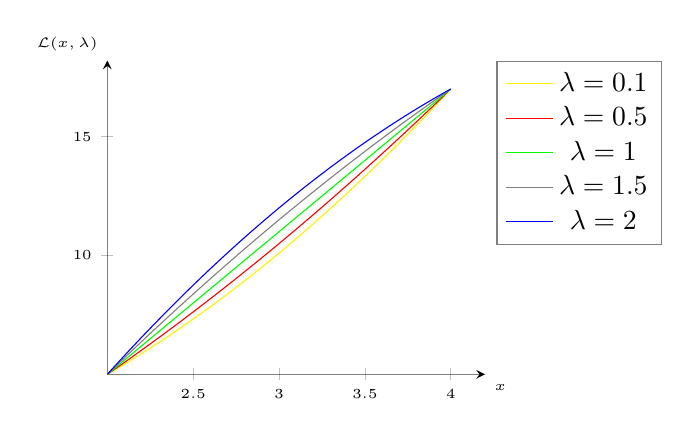
\begin{tikzpicture}
		    \begin{axis}[scale=.7,draw opacity =.5,samples=100,smooth, 
		      axis x line=center, 
		      axis y line=center,
		      ylabel = {$\mathcal{L}(x,\lambda)$},
		      xlabel = {$x$},
		      xlabel style={below right},
		      ylabel style={above left},
		      label style={font=\tiny},
		      tick label style={font=\tiny},
		      enlargelimits=upper,
		      legend pos=outer north east] 
		      \addplot[yellow,opacity=1,domain=2:4]{x^2 + 1 - .1*(x-2)*(x-4)};
		      \addlegendentry{$\lambda=0.1$}
		      \addplot[red,opacity=1,domain=2:4]{x^2 + 1 - .5*(x-2)*(x-4)};
		      \addlegendentry{$\lambda=0.5$}
		      \addplot[green,opacity=1,domain=2:4]{x^2 + 1 - 1*(x-2)*(x-4)};
		      \addlegendentry{$\lambda=1$}
		      \addplot[gray,opacity=1,domain=2:4]{x^2 + 1 - 1.5*(x-2)*(x-4)};
		      \addlegendentry{$\lambda=1.5$}
		      \addplot[blue,opacity=1,domain=2:4]{x^2 + 1 - 2*(x-2)*(x-4)};
		      \addlegendentry{$\lambda=2$}
		    \end{axis}
		\end{tikzpicture}
	    \end{center}
	    \vspace{.5cm}

	    Ahora, para encontrar el mínimo de $\mathcal{L}(x,\lambda)$ con respecto a $x$, tomamos la derivada de $\mathcal{L}$ con respecto a $x$ e igualamos a cero, obteniendo 
	    $$x = \frac{3\lambda}{\lambda - 2}.$$ 

	    Sin embargo, debido a la restricción $(x-2)(x-4) \leq 0$, $x$ debe estar en el intervalo $[2,4]$. Por lo tanto, el mínimo de $\mathcal{L}(x,\lambda)$ en el intervalo $[2,4]$ se alcanza en uno de los extremos del intervalo, es decir, en 
	    $$x=2\quad \text{o}\quad x=4.$$

	    Sustituyendo $x=2$ y $x=4$ en $\mathcal{L}(x,\lambda)$ obtenemos 
	    $$\mathcal{L}(2,\lambda) = 5\quad \text{y}\quad \mathcal{L}(4,\lambda) = 17.$$ 
	    Por lo tanto, el valor mínimo de $\mathcal{L}(x,\lambda)$ para $\lambda \leq 0$ y $x \in [2,4]$ es 5, que se alcanza en $x=2$.\\

	    Finalmente, el valor óptimo del problema de optimización original, $p^*$, es el valor mínimo de la función objetivo $x^2 + 1$ sujeto a la restricción $(x-2)(x-4) \leq 0$, que también es 5. Por lo tanto, podemos verificar que 
	    $$p^* = 5 \geq \inf_x \mathcal{L}(x,\lambda) = 5$$ 

	    para $\lambda \leq 0$, lo que verifica la desigualdad. Esto es consistente con la teoría de la optimización, que establece que el valor óptimo de un problema de optimización siempre es mayor o igual que el valor mínimo de su función Lagrangiana correspondiente para cualquier $\lambda \leq 0$.\\




	    La función dual de Lagrange, también conocida como función dual, se obtiene al minimizar la función Lagrangiana con respecto a las variables primales (en este caso, $x$) y luego maximizar con respecto a las variables duales (en este caso, $\lambda$). En otras palabras, la función dual $g(\lambda)$ se define como:
	    $$g(\lambda) = \inf_x \mathcal{L}(x,\lambda)$$

	    donde $\mathcal{L}(x,\lambda)$ es la función Lagrangiana. Para este problema, la función Lagrangiana es:
	    $$\mathcal{L}(x,\lambda) = x^2 + 1 - \lambda[(x-2)(x-4)]$$

	    Para encontrar $g(\lambda)$, primero minimizamos $\mathcal{L}(x,\lambda)$ con respecto a $x$. Como hemos resuelto anteriormente, el mínimo de $\mathcal{L}(x,\lambda)$ en el intervalo $[2,4]$ se alcanza en $x=2$ y su valor es 5. Por lo tanto, la función dual de Lagrange para este problema es una constante:
	    $$g(\lambda) = 5$$

	    para $\lambda \leq 0$. Esto significa que el valor óptimo del problema dual es $5$, que es igual al valor óptimo del problema primal. Esto es consistente con la teoría de la optimización, que establece que bajo ciertas condiciones (llamadas condiciones de Slater), el valor óptimo del problema primal es igual al valor óptimo del problema dual. Esto se conoce como dualidad fuerte.



	% ---------- (c)
	\item \textbf{\boldmath Describe el problema dual y comprueba que se trata de un problema de maximización cóncavo. Encuentra el valor dual óptimo $d^+$ y la solución dual óptima $\lambda^*$ ¿Se verifica la dualidad fuerte? Representa el conjunto $G\subset \mathbb{R}^2$}.\\

	    \textbf{Solución:}

    \end{enumerate}

    % -------------------- Ejercicio 2 -------------------- %
    \item \textbf{\boldmath ¿Cuáles son las condiciones de Slater asociadas al problema lineal
    $$
    \begin{array}{ll}
	\text{minimiza} & x^Tx\\
	\text{sujeto a} & Ax=b?
    \end{array}
    $$
    Se sabe que las condiciones de Slater implican que se verifica la dualidad fuerte. Describe esta situación para el problema lineal planteado. ¿Es posible aplicar las condiciones de Slater al problema 1?}\\

	\textbf{Solución:}

\end{comment}


    % -------------------- Ejercicio 3 -------------------- %
    \item \textbf{\boldmath Considera el problema de optimización
    $$
    \begin{array}{ll}
	\text{minimiza} & e^{-x}\\
	\text{sujeto a} & x^2/y\leq 0,\\
    \end{array}
    $$
    con variables $x$ e $y$, y dominio $D=\left\{(x,y):y>0\right\}$.}
    \begin{enumerate}[\bfseries (a)]

	% ---------- (a)
	\item \textbf{\boldmath Comprueba que es un problema de optimización convexa. Encuentra el valor óptimo}\\

	    \textbf{Solución:} Para demostrar que el problema de optimización dado es convexo y encontrar el valor óptimo, necesitamos verificar dos cosas: la convexidad de la función objetivo y la convexidad de las restricciones.\\

	    \textit{Convexidad de la función objetivo.-} La función objetivo es 
	    $$f(x) = e^{-x}.$$ 
	    Para demostrar que es convexa, necesitamos mostrar que su segunda derivada es siempre no negativa 
	    \footnote{
		Una función $f: \mathbb{R} \rightarrow \mathbb{R}$ es convexa en un intervalo $I$ si para todo $x \in I$, la segunda derivada $f''(x)$ existe y $f''(x) \geq 0$. En otras palabras, si la segunda derivada de una función es siempre no negativa en su dominio, entonces la función es convexa en ese dominio. Esto se debe a que la segunda derivada de una función mide la curvatura de la función, y una curvatura no negativa implica que la función es convexa.
	    }. 

	    Empecemos calculando la primera derivada de $f(x)$ que se obtiene utilizando la regla de la cadena para la derivación. La derivada de $e^u$ con respecto a $u$ es $e^u$, y la derivada de $-x$ con respecto a $x$ es $-1$. Por lo tanto, la primera derivada de $f(x)$ es:
	    $$f'(x) = \frac{d}{dx} e^{-x} = -e^{-x}.$$

	    La segunda derivada de $f(x)$ se obtiene derivando $f'(x)$ con respecto a $x$. Nuevamente, utilizamos la regla de la cadena. La derivada de $e^u$ con respecto a $u$ es $e^u$, y la derivada de $-x$ con respecto a $x$ es $-1$. Por lo tanto, la segunda derivada de $f(x)$ es:
	    $$f''(x) = \frac{d}{dx} (-e^{-x}) = e^{-x}.$$

	    Sabiendo que una función es convexa si su segunda derivada es siempre no negativa. La segunda derivada de $f(x)$ es $f''(x) = e^{-x}$, que es siempre positiva para todo $x$ en el dominio de los números reales, ya que la función exponencial $e^{-x}$ es siempre positiva. Por lo tanto, la función objetivo $f(x) = e^{-x}$ es convexa.\\

	    \textit{Convexidad de las restricciones.-} Sea la restricción,
	    $$g(x,y) = x^2/y \leq 0.$$ 
	     Ya que $y > 0$ (según $D=\left\{(x,y):y>0\right\}$), esta restricción implica que 
	     $$x = 0.$$ 

	    Un conjunto que consiste en un solo punto (en este caso, el punto $x = 0$) es un conjunto convexo. Esto se debe a que para cualquier par de puntos en el conjunto (que en este caso son el mismo punto $x = 0$), el segmento de línea que los conecta también está en el conjunto. Por lo tanto, la restricción $g(x,y) = x^2/y \leq 0$ define un conjunto convexo.\\

	    Así, el problema de optimización dado es convexo.\\

	    Para encontrar el valor óptimo del problema de optimización dado, debemos evaluar la función objetivo en el punto que satisface la restricción. Es decir, debemos evaluar la función objetivo en $x = 0$. Haciendo esto, obtenemos:
	    $$f(0) = e^{-0} = e^0 = 1.$$

	    Por lo tanto, el valor óptimo del problema de optimización dado es $1$.

	    Este resultado se obtiene al considerar que la función objetivo $f(x)$ es decreciente
	    \footnote{
		La función objetivo en este problema de optimización es $f(x) = e^{-x}$. Esta es una función exponencial decreciente para $x \geq 0$, lo que significa que a medida que $x$ aumenta, $f(x)$ disminuye.\\
	    }
	    para $x \geq 0$ y la restricción implica que $x = 0$. Por lo tanto, el valor mínimo de $f(x)$, llamémoslo $p^*$ en el dominio dado es 
	    $$p^*=f(0) = e^0 = 1.$$\\


	% ---------- (b)
	\item \textbf{\boldmath Establece el problema dual y encuentra la solución óptima dual $\lambda^*$ y el valor óptimo $d^*$. ¿Cuál es el salto de dualidad $p^*-d^*$? Representa el conjunto $G\subseteq \mathbb{R}^2$.}\\

	    \textbf{Solución:} Veamos que el problema de optimización primal es:
	    $$
	    \left\{
		\begin{array}{ll}
			\text{minimiza} & e^{-x}\\
			\text{sujeto a} & x^2/y\leq 0,\\
		\end{array}
	    \right.
	    $$

	    con variables $x$ e $y$, y dominio $D=\left\{(x,y):y>0\right\}$.\\

	    Para formular el problema dual, primero expresamos el problema primal en su forma estándar. Sean la función objetivo $f_0(x) = e^{-x}$ y la restricción $f_1(x,y) = x^2/y \leq 0$. Entonces, el problema primal podemos escribir como:
	    $$
	    \left\{
		\begin{array}{ll}
			\text{minimiza} & f_0(x)\\
			\text{sujeto a} & f_1(x,y) \leq 0,\\
		\end{array}
	    \right.
	    $$

	    Luego, procedamos a formular el problema dual. Para ello, necesitamos definir la función Lagrangiana, que incorpora las restricciones del problema primal en la función objetivo a través de las variables duales. En este caso, la función Lagrangiana se define como:
	    $$
	    L(x,y,\lambda) = f_0(x) + \lambda f_1(x,y) = e^{-x} + \lambda \left(\frac{x^2}{y}\right)
	    $$

	    donde $\lambda$ es la variable dual asociada a la restricción $f_1(x,y) \leq 0$.\\

	    La función dual de Lagrange, que es la función objetivo del problema dual, se obtiene al minimizar la función Lagrangiana con respecto a las variables primales. Es decir, buscamos el valor mínimo de la función Lagrangiana sobre todas las posibles elecciones de las variables primales $x$ e $y$. En decir, por el método de los multiplicadores de Lagrange, tenemos:
	    $$
	     \inf_{x,y} L(x,y,\lambda) = \inf_{x,y} \left[e^{-x} + \lambda \left(\frac{x^2}{y}\right)\right]=g(\lambda).
	    $$

	    Para resolverlo, tomamos las derivadas parciales de $L$ con respecto a $x$ e $y$, 
	    $$
	    \left\{
		\begin{array}{rcl}
		    \dfrac{\partial L}{\partial x} &=& -e^{-x} + 2\lambda \dfrac{x}{y}\\\\
		    \dfrac{\partial L}{\partial y} &=& -\lambda \dfrac{x^2}{y^2}.
		\end{array}
	    \right.
	    $$

	    Igualando estas derivadas a cero,
	    $$
	    \left\{
		\begin{array}{rcl}
		    -e^{-x} + 2\lambda \frac{x}{y} &=& 0\\\\
		    -\lambda \frac{x^2}{y^2} &=& 0,
		\end{array}
	    \right.
	    $$
	    Y sabiendo que $y > 0$, obtenemos, 
	    $$x = 0.$$
	    Por lo tanto, la función dual de Lagrange es:
	    $$
	    g(\lambda) = \inf_{x,y} L(x,y,\lambda) = \inf_{x,y} \left[e^{-x} + \lambda \left(\frac{x^2}{y}\right)\right] = e^{-0} + \lambda \left(\frac{0^2}{y}\right) = 1.
	    $$
	    para $\lambda \geq 0$.\\

	    Así, dado que $g(\lambda)$ es constante e igual a $1$ para todo $\lambda \geq 0$, la solución óptima dual $\lambda^*$ puede ser cualquier número real no negativo y el valor óptimo dual 
	    $$d^* = g(\lambda^*) = 1.$$

	    Finalmente, puedes calcular la brecha de dualidad $p^*-d^*$, donde $p^*$ es el valor óptimo del problema primal. Dado que $p^* = d^* = 1$, la brecha de dualidad es $0$.\\\\

	% ---------- (c)
	\item \textbf{\boldmath ¿Se cumple la condición de Slater para este problema?.}\\

	    \textbf{Solución:} La condición de Slater es una regla que se utiliza en optimización convexa. Esta regla dice que si hay un punto que cumple todas las restricciones del problema de optimización de manera estricta, entonces podemos estar seguros de que la solución óptima del problema original (llamado problema primal) y la solución óptima del problema asociado (llamado problema dual) serán iguales. Esto se conoce como dualidad fuerte.\\

	    En este caso, el problema de optimización tiene una restricción que dice que $x^2/y\leq 0$ y que $y>0$. Esto significa que $x=0$ para cualquier par $(x,y)$ que cumpla $y>0$. Por lo tanto, el punto $(0,1)$ cumple la restricción de manera estricta, ya que $0^2/1=0$ es estrictamente menor que 0.\\

	    Por lo tanto, la condición de Slater se cumple para este problema de optimización. Esto significa que la solución óptima del problema original y la solución óptima del problema dual son iguales, lo cual es consistente con los cálculos anteriores donde encontramos que ambas soluciones óptimas son 1. Es decir, no hay diferencia o brecha entre las soluciones óptimas del problema original y del problema dual.\\\\


    \end{enumerate}

    % -------------------- Ejercicio 4 -------------------- %
    \item \textbf{\boldmath Considera el problema:
    $$
    \begin{array}{ll}
	\text{minimiza} & f_0(x)\\
	\text{sujeto a} & f_i(x)\leq 0, \; i=1,\dots,m\\
    \end{array}
    $$
    donde las funciones $f_i:\mathbb{R}^n\to \mathbb{R}$ son diferenciables y convexas. Muestra que la función
    $$\phi(x) = f_0(x)+\alpha \sum_{i=1}^m \max\left\{0,f_i(x)\right\}^2,$$
    es convexa (cuando $\alpha>0)$. Si $\tilde{x}$ minimiza $\phi$, muestra cómo obtener, a partir de $\tilde{x}$, un punto accesible para el problema dual. Encuentra la cota inferior correspondiente al problema primal.}\\

	\textbf{Solución:} Para demostrar que la función $$\phi(x) = f_0(x)+\alpha \sum_{i=1}^m \max\left\{0,f_i(x)\right\}^2$$ es convexa cuando $\alpha>0$, necesitamos mostrar que para cualquier $x, y \in \mathbb{R}^n$ y cualquier $t \in [0,1]$, se cumple que:
$$\phi(tx + (1-t)y) \leq t\phi(x) + (1-t)\phi(y).$$

Sea $f_0(x)$  convexa. Entonces, sabemos que:
$$f_0(tx + (1-t)y) \leq tf_0(x) + (1-t)f_0(y).$$

Además, la función $\max\{0, f_i(x)\}^2$ es convexa porque es la composición de una función convexa no decreciente $\left(x^2\right)$ y una función convexa $\left(\max\{0, f_i(x)\}\right)$. Por lo tanto, para cada $i$:
$$\max\{0, f_i(tx + (1-t)y)\}^2 \leq t\max\{0, f_i(x)\}^2 + (1-t)\max\{0, f_i(y)\}^2.$$

Sumando estas desigualdades para todos los $i$ y multiplicando por $\alpha$, obtenemos:
$$\alpha \sum_{i=1}^m \max\{0, f_i(tx + (1-t)y)\}^2 \leq \alpha \sum_{i=1}^m \left[ t\max\{0, f_i(x)\}^2 + (1-t)\max\{0, f_i(y)\}^2 \right].$$

Finalmente, sumando las dos desigualdades anteriores, obtenemos la desigualdad deseada:
$$
\begin{array}{rcl}
    \phi(tx + (1-t)y) &=& \displaystyle f_0(tx + (1-t)y) + \alpha \sum_{i=1}^m \max\{0, f_i(tx + (1-t)y)\}^2\\\\
		      &\leq& \displaystyle f_0(x) + (1-t)f_0(y) + \alpha \sum_{i=1}^m \left[ t\max\{0, f_i(x)\}^2 + (1-t)\max\{0, f_i(y)\}^2 \right]\\\\
		      &=& \displaystyle t\left[ f_0(x) + \alpha \sum_{i=1}^m \max\{0, f_i(x)\}^2 \right] + (1-t)\left[ f_0(y) + \alpha \sum_{i=1}^m \max\{0, f_i(y)\}^2 \right]\\\\
		      &=& t\phi(x) + (1-t)\phi(y).
\end{array}
$$

Por lo tanto, $\phi(x)$ es convexa cuando $\alpha > 0$.\\\\


    % -------------------- Ejercicio 5 -------------------- %
    \item \textbf{\boldmath Minimizando una función cuadrática. Considera el problema de minimizar una función cuadrática:
    $$\text{minimiza} \; f(x)=(1/2)x^TPx+q^Tx+r,$$
    donde $P$ es una matriz simétrica (no necesariamente en $S^n_{+}$).}\\

    \begin{enumerate}[(a)]

	% ---------- (a)
	\item \textbf{\boldmath Muestra que si $P \nsucceq 0$ (es decir, la función no es convexa) entonces el problema no está acotado inferiormente.}\\

	    \textbf{Solución:} Vamos a demostrar que si la matriz $P$ de una función cuadrática no es semidefinida positiva (es decir, $P\nsucceq0$), entonces la función no está acotada inferiormente. Para ello, vamos a utilizar un argumento de reducción al absurdo.\\

	    Supongamos que la función cuadrática 
	    $$f(x) = \frac{1}{2}x^TPx + q^Tx + r$$
	    está acotada inferiormente con $P \nsucceq 0$. Esto implicaría que existe un número real $M$ tal que 
	    $$f(x) \geq M$$ 
	    para todo $x$. Sin embargo, debido a que $P \nsucceq 0$, lo cual significa que $P$ no es una matriz semidefinida positiva, sabemos por definición que existe un vector $x$ tal que 
	    $$x^TPx < 0.$$

	    Si escalamos este vector por un escalar grande $\alpha$, la expresión $\alpha^2 x^TPx$ se vuelve arbitrariamente negativa. Esto se debe a que si $x^TPx < 0$, entonces $\alpha^2 x^TPx$ será aún más negativo a medida que $\alpha$ se haga más grande.\\

	    Elijamos $\alpha$ de manera que la función $f(\alpha x)$ sea menor que cualquier cota inferior dada. Sea, $f(\alpha x)$ 
	    $$f(\alpha x) = \frac{1}{2}\alpha^2 x^TPx + \alpha q^Tx + r.$$ 

	    Luego, hacemos que esta función sea menor que $-M$. Es decir, 
	    $$\frac{1}{2}\alpha^2 x^TPx + \alpha q^Tx + r < -M.$$ 

	    Multiplicamos ambos lados de la desigualdad por 2,
	    $$\alpha^2 x^TPx + 2\alpha q^Tx + 2r < -2M.$$ 

	    Reorganizando los términos,  
	    $$\alpha^2 x^TPx < -2M - 2\alpha q^Tx - 2r.$$ 

	    Esto garantiza que el término cuadrático en $f(\alpha x)$ sea suficientemente negativo para compensar los otros términos en $f(\alpha x)$ y hacer que toda la función sea menor que $-M$.

	    Por lo tanto, encontramos que 
	    $$f(\alpha x) = \frac{1}{2}\alpha^2 x^TPx + \alpha q^Tx + r < -M,$$

	    lo cual contradice nuestra suposición inicial de que $f(x)$ está acotada inferiormente. Por lo tanto, si $P \nsucceq 0$, la función cuadrática $f(x)$ no puede estar acotada inferiormente. \\\\

	% ---------- (b)
	\item \textbf{\boldmath Si suponemos que $P \succeq 0$, pero que la condición de optimalidad $Px^* = -q$ no tiene solución. Muestra que el problema vuelve a no estar acotado inferiormente.}\\

	    \textbf{Solución:} Si suponemos que $P \succeq 0$ (es decir, $P$ es semidefinida positiva), pero la condición de optimalidad $Px^* = -q$ no tiene solución, entonces podemos demostrar que el problema de minimización no está acotado inferiormente.\\

	    La condición de optimalidad $Px^* = -q$ proviene de tomar el gradiente de la función cuadrática $f(x)$ y establecerlo igual a cero. Si esta ecuación no tiene solución, significa que no existe un punto $x^*$ en el cual el gradiente de $f(x)$ sea cero. En otras palabras, no existe un mínimo local para la función.\\

	    Dado que $P \succeq 0$, la función cuadrática $f(x)$ es convexa. Para una función convexa, cualquier mínimo local es también un mínimo global. Entonces, si no existe un mínimo local para la función (es decir, no existe un punto en el que el gradiente de la función sea cero), la función no tiene un mínimo global. Esto se debe a que un mínimo global para una función es un punto para el cual la función no toma valores menores. En otras palabras, no existe ningún otro punto en el dominio de la función donde el valor de la función sea menor. Si no existe tal punto, entonces la función no tiene un mínimo global. Esto significa que la función no está acotada inferiormente, ya que una función está acotada inferiormente si existe un número real tal que para todo valor en el dominio, el valor de la función es mayor o igual a ese número. Si no existe tal número, entonces la función no está acotada inferiormente.\\

	    Por lo tanto, si suponemos que $P \succeq 0$, pero que la condición de optimalidad $Px^* = -q$ no tiene solución, entonces el problema de minimización no está acotado inferiormente. Esto concluye la demostración.\\\\

    \end{enumerate}

    % -------------------- Ejercicio 6 -------------------- %
    \item \textbf{\boldmath Considera el problema siguiente:
    $$\text{minimiza} \; f(x)=(1/2)\left(x_1^2+\gamma x^2_2\right),\; \gamma >0.$$} 
    \begin{enumerate}[\bfseries (a)]

	% ---------- (a)
	\item \textbf{\boldmath Fija $(a,b)\in \mathbb{R}^2$. Calcula el valor de $t$ que minimiza la función $f\left((a,b)-t\nabla f(a,b)\right)$ en términos de $a$ y $b$, claro.}\\ 

	    \textbf{Solución:} Teniendo en cuenta que estamos trabajando en $\mathbb{R}^2$ y que $\gamma > 0$:

	    Consideremos la función $$f: \mathbb{R}^2 \rightarrow \mathbb{R}$$ definida por $$f(x) = \frac{1}{2}(x_1^2 + \gamma x_2^2),$$ donde $x = (x_1, x_2)$ es un vector en $\mathbb{R}^2$ y $\gamma > 0$ es una constante.\\

	    Sabemos que el gradiente de una función es un vector que apunta en la dirección en la que la función aumenta más rápidamente. En otras palabras, si estamos en un punto en el espacio y queremos saber en qué dirección debemos movernos para aumentar el valor de la función lo más rápido posible, debemos movernos en la dirección del gradiente.\\

	    Para calcular el gradiente de esta función, tomamos las derivadas parciales de la función con respecto a cada una de las variables, $x_1$ y $x_2$. 

	    La derivada parcial de $f$ con respecto a $x_1$ es la derivada de $\frac{1}{2}x_1^2$ con respecto a $x_1$, manteniendo $x_2$ constante. Como la derivada de $x_1^2$ con respecto a $x_1$ es $2x_1$, la derivada parcial de $f$ con respecto a $x_1$ es 
	    $$x_1.$$ 
	    De manera similar, la derivada parcial de $f$ con respecto a $x_2$ es la derivada de $\frac{1}{2}\gamma x_2^2$ con respecto a $x_2$, manteniendo $x_1$ constante. Como la derivada de $\gamma x_2^2$ con respecto a $x_2$ es $2\gamma x_2$, la derivada parcial de $f$ con respecto a $x_2$ es 
	    $$\gamma x_2.$$

	    Por lo tanto, el gradiente de $f$ es 
	    $$(x_1, \gamma x_2).$$

	    Así, el gradiente de la función en el punto $(a,b)$ en $\mathbb{R}^2$ es 
	    $$\nabla f(a,b) = (a, \gamma b).$$

	    Esto significa que si estás en el punto $(a,b)$ en $\mathbb{R}^2$, la dirección en la que la función $f(x)$ aumenta más rápidamente es en la dirección del vector $(a, \gamma b)$.\\

	    Consideremos ahora un paso de gradiente desde el punto $(a,b)$ en la dirección opuesta al gradiente 
	    \footnote{
		Recordemos que una forma de minimizar una función es a través de un proceso llamado "descenso de gradiente". La idea es comenzar en un punto inicial y luego moverse repetidamente en la dirección que disminuye la función más rápidamente, que es la dirección opuesta al gradiente. Entonces, cuando decimos que el punto $(a,b)$ es "desplazado" por $-t\nabla f(a,b)$, lo que realmente queremos decir es que estamos moviendo el punto $(a,b)$ una pequeña cantidad en la dirección que disminuye la función más rápidamente. El tamaño de este movimiento está determinado por $t$, y la dirección de este movimiento está determinada por el gradiente $\nabla f(a,b)$.
		Por lo tanto, $(a,b)-t\nabla f(a,b)$ representa el nuevo punto después de dar un paso de gradiente de tamaño $t$ desde el punto $(a,b)$ en la dirección opuesta al gradiente.\\}. 
	    Este paso se puede representar como 
	    $$(a,b)-t\nabla f(a,b)=(a,b)-t(a,\gamma b),$$ 

	    donde $t$ es el valor que minimiza la función.\\

	    Vamos a calcular el valor de $t$ que minimiza la función $f\left((a,b)-t\nabla f(a,b)\right)$ 
	    \footnote{ El valor de $t$ se calcula en la función $f$ porque estamos buscando el valor que minimiza la función $f$ después de un paso de gradiente.}. 
	    Para hacer esto, primero necesitamos expresar la función $f$ en términos de $t$. Sustituyendo $(a,b)-t\nabla f(a,b)$ en $f$, obtenemos
	    $$
	    \begin{array}{rcl}
	    f\left((a,b)-t\nabla f(a,b)\right) &=& f\left((a,b)-t(a,\gamma b)\right)\\\\
					       &=& f\left((a-ta, b-t\gamma b)\right)\\\\
					       &=& \dfrac{1}{2}\left((a-ta)^2 + \gamma (b-t\gamma b)^2\right).
	    \end{array}
	    $$

	    Ahora, encontremos el valor de $t$ que minimiza la función.  Primero, tenemos la derivada de la función $f\left((a,b)-t\nabla f(a,b)\right)$ con respecto a $t$:
	    $$\frac{df}{dt} = -(a^2 - 2a^2t + \gamma b^2 - 2\gamma^2 b^2t).$$

	    Para encontrar el valor de $t$ que minimiza la función, necesitamos igualar esta derivada a cero. Esto nos da la ecuación:
	    $$-(a^2 - 2a^2t + \gamma b^2 - 2\gamma^2 b^2t) = 0.$$

	    Podemos simplificar esta ecuación distribuyendo el signo negativo a través de los términos en el paréntesis:
	    $$-a^2 + 2a^2t - \gamma b^2 + 2\gamma^2 b^2t = 0.$$

	    Luego, reorganizamos los términos para agrupar los términos que contienen $t$:
	    $$2a^2t + 2\gamma^2 b^2t = a^2 + \gamma b^2.$$

	    Factorizamos $t$ del lado izquierdo de la ecuación:
	    $$t(2a^2 + 2\gamma^2 b^2) = a^2 + \gamma b^2.$$

	    por lo tanto, para cualquier par de puntos $(a,b)\in \mathbb{R}^2$ y $\gamma>0$ el valor de $t$ que minimiza la función $f\left((a,b)-t\nabla f(a,b)\right)$ es
	    $$t = \frac{a^2 + \gamma b^2}{2a^2 + 2\gamma^2 b^2}.$$\\\\


	% ---------- (b)
	\item \textbf{\boldmath Crea un programa en MATLAB o Python tal que:}

	    \begin{itemize}

		\item \textbf{\boldmath Tenga como entrada: el parámetro $\gamma$, una tolerancia $\epsilon$, un número máximo de iteraciones $N$ y un punto inicial $\left(x_1^{(0)},x_2^{(0)}\right)$.}\\

		\item \textbf{Aplique el método del gradiente al problema, utilizando paso exacto (obtenido en el apartado (a)).}\\

		\item \textbf{\boldmath Que pare cuando llegue al número máximo de iteraciones o cuando la precisión sea menor que $\epsilon$.}\\

		\item \textbf{El problema debe devolver la última aproximación y el número de iteraciones utilizado, así como un mensaje que informe de los posibles fallos producidos y de la condición de parada utilizada.}\\

	    \end{itemize}


	% ---------- (c)
	\item \textbf{Si te sientes con ganas, añade la funcionalidad de que al terminar represente el conjunto inicial $S$, las curvas de nivel por las que pasa cada aproximación, destacando el punto aproximado con un dot.}\\

	    \textbf{Solución de (b) y (c):}
\begin{lstlisting}[language=Python]
import numpy as np
import matplotlib.pyplot as plt
from matplotlib.colors import LogNorm

def gradient_descent(gamma, epsilon, N, initial_point):
    # Item 1: La funcion toma como entrada el parametro gamma,
    # una tolerancia epsilon,  un numero maximo de iteraciones N 
    # y un punto inicial (x1(0), x2(0)).
    
    # Definimos la funcion y su gradiente
    f = lambda x: 0.5 * (x[0]**2 + gamma*x[1]**2)
    grad_f = lambda x: np.array([x[0], gamma*x[1]])

    # Inicializamos el punto y el numero de iteraciones
    x = np.array(initial_point)
    num_iterations = 0

    # Creamos una lista para almacenar todas las aproximaciones
    approximations = [x]

    # Bucle principal del metodo del gradiente
    while num_iterations < N:
        # Item 2: Aplicamos el metodo del gradiente al problema, 
	# utilizando paso exacto.
        # Calculamos el gradiente
        gradient = grad_f(x)

        # Calculamos el tamano del paso
        t = (x[0]**2+gamma*x[1]**2)/(2*x[0]**2+2*gamma**2*x[1]**2)

        # Actualizamos el punto
        x = x - t * gradient

        # Anadimos la nueva aproximacion a la lista
        approximations.append(x)

        # Item 3: El bucle continua hasta que se alcanza el numero
	# maximo de iteraciones o hasta que la norma del gradiente 
	# es menor que epsilon.
        if np.linalg.norm(gradient) < epsilon:
            print("El algoritmo  convergio con exito.")
            break

        # Actualizamos el numero de iteraciones
        num_iterations += 1

    # Item 4: La funcion devuelve la ultima aproximacion al minimo 
    # de la funcion y el numero de iteraciones que se utilizaron. 
    # Tambien se imprime un mensaje que informa de los posibles
    # fallos producidos y de la condicion de parada que se utilizo.
    if num_iterations == N:
        print("El algoritmo convergio en el numero maximo de iter.")
    else:
        print("El algoritmo convergio con exito.")

    # Creamos una cuadricula de puntos en el espacio 2D
    y = np.linspace(-10, 10, 400)
    x = np.linspace(-10, 10, 400)
    X, Y = np.meshgrid(x, y)

    # Calculamos los valores de la funcion en cada punto de la 
    # cuadricula
    Z = 0.5 * (X**2 + gamma*Y**2)

    # Creamos una figura y un conjunto de ejes en matplotlib
    fig, ax = plt.subplots()
    
    # Dibujamos las curvas de nivel de la funcion
    ax.contour(X, Y, Z, 
	       levels=np.logspace(0, 5, 35), 
	       norm=LogNorm(), 
	       cmap=plt.cm.jet)

    # Convertimos la lista de aproximaciones en un array de 
    # numpy para facilitar su manejo
    approximations = np.array(approximations)

    # Dibujamos los puntos aproximados
    ax.plot(approximations[:, 0], approximations[:, 1], 'ko')

    # Mostramos la figura
    plt.show()

    return x, num_iterations
\end{lstlisting}
    \end{enumerate}


\end{enumerate}
